\documentclass{standalone}

\usepackage{pgf,tikz,pgfplots,pgfplotstable}

% for patch type=bilinear
\usepgfplotslibrary{patchplots}

\begin{document}

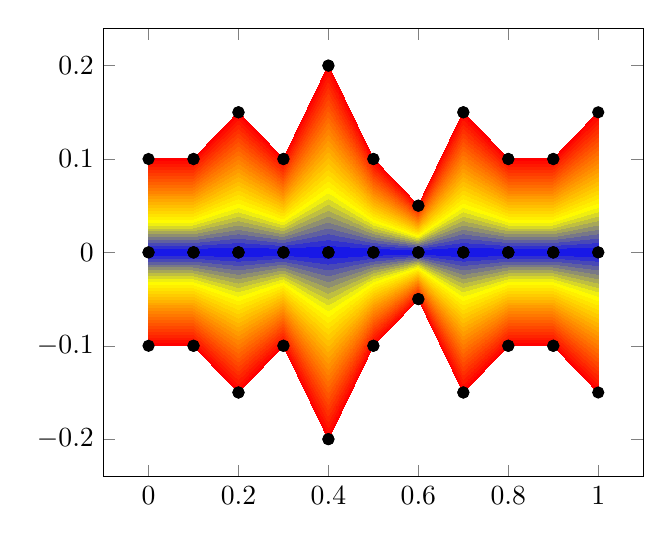
\begin{tikzpicture}%[scale=5]

\def\image{%
    \begin{axis}[
        point meta=explicit,
    ]
	\addplot [ 
		shader=interp, 
		patch, 
		patch type=bilinear, 
		mark=*, 
	]
	coordinates {
		(0.0,0.1) [1] (0.0,0) [0] (0.1,0) [0] (0.1,0.1) [1] 
		(0.0,-0.1) [1] (0.0,0) [0] (0.1,0) [0] (0.1,-0.1) [1] 
		
		(0.1,0.1) [1] (0.1,0) [0] (0.2,0) [0] (0.2,0.15) [1] 
		(0.1,-0.1) [1] (0.1,0) [0] (0.2,0) [0] (0.2,-0.15) [1] 
		
		(0.2,0.15) [1] (0.2,0) [0] (0.3,0) [0] (0.3,0.1) [1] 
		(0.2,-0.15) [1] (0.2,0) [0] (0.3,0) [0] (0.3,-0.1) [1] 
		
		(0.3,0.1) [1] (0.3,0) [0] (0.4,0) [0] (0.4,0.2) [1] 
		(0.3,-0.1) [1] (0.3,0) [0] (0.4,0) [0] (0.4,-0.2) [1] 
		
		(0.4,0.2) [1] (0.4,0) [0] (0.5,0) [0] (0.5,0.1) [1] 
		(0.4,-0.2) [1] (0.4,0) [0] (0.5,0) [0] (0.5,-0.1) [1] 
		
		(0.5,0.1) [1] (0.5,0) [0] (0.6,0) [0] (0.6,0.05) [1] 
		(0.5,-0.1) [1] (0.5,0) [0] (0.6,0) [0] (0.6,-0.05) [1] 
		
		(0.6,0.05) [1] (0.6,0) [0] (0.7,0) [0] (0.7,0.15) [1] 
		(0.6,-0.05) [1] (0.6,0) [0] (0.7,0) [0] (0.7,-0.15) [1]
		
		(0.7,0.15) [1] (0.7,0) [0] (0.8,0) [0] (0.8,0.1) [1]
		(0.7,-0.15) [1] (0.7,0) [0] (0.8,0) [0] (0.8,-0.1) [1]
		
		(0.8,0.1) [1] (0.8,0) [0] (0.9,0) [0] (0.9,0.1) [1]
		(0.8,-0.1) [1] (0.8,0) [0] (0.9,0) [0] (0.9,-0.1) [1]
		
		(0.9,0.1) [1] (0.9,0) [0] (1.0,0) [0] (1.0,0.15) [1] 
		(0.9,-0.1) [1] (0.9,0) [0] (1.0,0) [0] (1.0,-0.15) [1] 
	};
    \end{axis}
}%

%\begin{scope}[rotate around = {-90:(1,1)},shift={(1,1)}]
    \image
%\end{scope}

\end{tikzpicture}
\end{document}
